\section{The Phong Illumination Model}

\begin{frame}{Phong Model Overview}
    \begin{columns}
        \begin{column}{0.5\textwidth}
            \begin{conceptbox}{Historical Context}
                \textbf{Developed by:} Bui Tuong Phong (1975)
                
                \textbf{Goal:} Fast, realistic-looking lighting for computer graphics
                
                \vspace{0.3cm}
                \textbf{Key insight:} Break lighting into three components that can be computed independently
            \end{conceptbox}
            
            \vspace{0.3cm}
            \pause
            \begin{mathbox}{Complete Phong Formula}
                \begin{align}
                    I &= I_{\text{ambient}} + I_{\text{diffuse}} + I_{\text{specular}} \\
                    &= k_a I_a + k_d I_l (\mathbf{N} \cdot \mathbf{L}) + k_s I_l (\mathbf{R} \cdot \mathbf{V})^n
                \end{align}
            \end{mathbox}
        \end{column}
        \begin{column}{0.5\textwidth}
            \begin{tikzpicture}[scale=0.8]
                % Surface
                \draw[ObjectColor, very thick] (-2,0) -- (2,0);
                \fill[ObjectColor] (0,0) circle (3pt);
                
                % Normal vector
                \draw[->, PrimaryColor, thick] (0,0) -- (0,1.5);
                \node[right] at (0.1,0.75) {\footnotesize $\mathbf{N}$};
                
                % Light vector
                \draw[->, lightray, thick] (0,0) -- (-1.2,1.2);
                \node[above] at (-0.8,0.8) {\footnotesize $\mathbf{L}$};
                
                % View vector
                \draw[->, AccentColor, thick] (0,0) -- (1.2,1.2);
                \node[above] at (0.8,0.8) {\footnotesize $\mathbf{V}$};
                
                % Reflection vector
                \draw[->, reflectray, thick] (0,0) -- (1.2,1.2);
                \node[above right] at (1,1.4) {\footnotesize $\mathbf{R}$};
                
                % Angles
                \draw[dashed] (0,0) -- (0,1);
                \draw[dashed] (0,0) -- (-1,1);
                \node[PrimaryColor] at (-0.3,0.4) {\footnotesize $\theta_i$};
                
                \draw[dashed] (0,0) -- (0,1);
                \draw[dashed] (0,0) -- (1,1);
                \node[AccentColor] at (0.3,0.4) {\footnotesize $\theta_r$};
            \end{tikzpicture}
            
            \vspace{0.3cm}
            \pause
            % IMAGE: Three components breakdown
            % Show sphere with: ambient only, +diffuse, +specular
            % 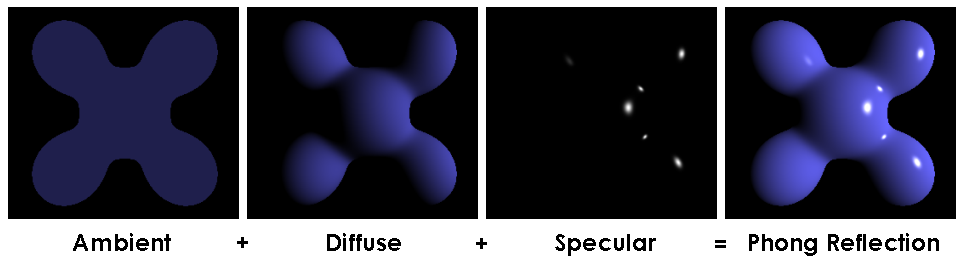
\includegraphics[width=\linewidth]{images/phong_components.jpg}
            \textcolor{gray}{[Phong components breakdown]}
        \end{column}
    \end{columns}
\end{frame>

\begin{frame}{Ambient Reflection - Theory}
    \begin{columns}
        \begin{column}{0.5\textwidth}
            \begin{raybox}{Ambient Light Motivation}
                \textbf{Problem:} In real life, shadows aren't completely black
                
                \vspace{0.3cm}
                \textbf{Causes:}
                \begin{itemize}
                    \item Light bounces off walls, ceiling
                    \item Atmospheric scattering
                    \item Multiple light sources
                    \item Diffuse skylight
                \end{itemize}
                
                \vspace{0.3cm}
                \textbf{Solution:} Add constant illumination everywhere
            \end{raybox>
        \end{column>
        \begin{column>{0.5\textwidth>
            \begin{tikzpicture>[scale=0.8]
                % Scene with indirect lighting
                \draw[thick] (0,0) rectangle (3,3);
                
                % Direct light source
                \node[circle, fill=LightColor, minimum size=0.6cm] (light) at (2.5,2.5) {};
                \draw[lightray] (light) -- (1.5,1.5);
                
                % Object in "shadow"
                \node[sphere, minimum size=0.8cm] (obj) at (0.8,0.8) {};
                
                % Bounced light rays (dashed)
                \draw[lightray, dashed, opacity=0.5] (3,1.5) -- (obj);
                \draw[lightray, dashed, opacity=0.5] (1.5,3) -- (obj);
                \draw[lightray, dashed, opacity=0.5] (0,2) -- (obj);
                
                \node[below] at (1.5,-0.3) {\footnotesize Even shadowed areas};
                \node[below] at (1.5,-0.6) {\footnotesize receive some light};
            \end{tikzpicture>
        \end{column>
    \end{columns>
    
    \vspace{0.3cm}
    \pause
    \begin{center>
        % IMAGE: Scene with and without ambient lighting
        % Show same scene: left without ambient (pure black shadows), right with ambient
        % \includegraphics[width=0.8\linewidth]{images/ambient_comparison.jpg}
        \textcolor{gray>{[Comparison: without ambient vs with ambient]}
    \end{center>
\end{frame>

\begin{frame}{Ambient Reflection - Mathematics}
    \begin{mathbox}{Ambient Component Formula}
        \textbf{Simplest lighting component:}
        \begin{align}
            I_{\text{ambient}} = k_a \cdot I_a
        \end{align}
        
        where:
        \begin{itemize}
            \item $k_a$ = ambient reflection coefficient of the material
            \item $I_a$ = intensity of ambient light in the scene
        \end{itemize}
        
        \vspace{0.3cm}
        \pause
        \textbf{Key properties:}
        \begin{itemize}
            \item Independent of viewer position
            \item Independent of light direction
            \item Independent of surface normal
            \item Same for all points on the surface
        \end{itemize>
        
        \vspace{0.3cm}
        \pause
        \textbf{Typical values:}
        \begin{itemize}
            \item $k_a$: 0.1 to 0.3 (material property)
            \item $I_a$: 0.1 to 0.2 (scene setting)
        \end{itemize>
    \end{mathbox>
    
    \vspace{0.3cm}
    \pause
    % IMAGE: Different ambient coefficients
    % Show spheres with ka = 0.0, 0.1, 0.3, 0.5
    % \includegraphics[width=\linewidth]{images/ambient_coefficients.jpg}
    \textcolor{gray}{[Effect of different ambient coefficients]}
\end{frame>

\begin{frame}{Diffuse Reflection - Introduction}
    \begin{columns}
        \begin{column}{0.5\textwidth}
            \begin{conceptbox}{Lambertian Surfaces}
                \textbf{Examples:}
                \begin{itemize}
                    \item Matte paint
                    \item Unpolished wood
                    \item Paper
                    \item Clay
                    \item Fabric
                \end{itemize>
                
                \vspace{0.3cm}
                \textbf{Characteristics:}
                \begin{itemize}
                    \item Surface appears equally bright from all viewing angles
                    \item Light scattered uniformly in all directions
                    \item Brightness depends only on angle of incident light
                \end{itemize>
            \end{conceptbox>
        \end{column>
        \begin{column>{0.5\textwidth>
            \begin{tikzpicture>[scale=0.8]
                % Surface with normal
                \draw[ObjectColor, very thick] (-2,0) -- (2,0);
                \fill[ObjectColor] (0,0) circle (3pt);
                \draw[->, PrimaryColor, thick] (0,0) -- (0,1.5);
                \node[right] at (0.1,0.75) {\footnotesize $\mathbf{N}$};
                
                % Light ray at angle
                \draw[->, lightray, thick] (-1.5,1.5) -- (0,0);
                \node[above] at (-0.75,0.75) {\footnotesize $\mathbf{L}$};
                
                % Angle between normal and light
                \draw[dashed] (0,0) -- (0,1);
                \draw[dashed] (0,0) -- (-1,1);
                \node[AccentColor] at (-0.3,0.4) {\footnotesize $\theta$};
                
                % Scattered rays (equal intensity in all directions)
                \foreach \angle in {30,60,90,120,150} {
                    \draw[reflectray, opacity=0.6] (0,0) -- (\angle:1);
                }
                
                \node[below] at (0,-0.5) {\footnotesize Equal brightness};
                \node[below] at (0,-0.8) {\footnotesize all directions};
            \end{tikzpicture>
        \end{column>
    \end{columns>
    
    \vspace{0.3cm}
    \pause
    \begin{center>
        % IMAGE: Lambertian material examples
        % Show photos of matte surfaces: paper, clay pot, matte paint
        % \includegraphics[width=0.8\linewidth]{images/lambertian_examples.jpg}
        \textcolor{gray>{[Examples of Lambertian materials]}
    \end{center>
\end{frame>

\begin{frame}{Lambert's Cosine Law - Geometric Derivation}
    \begin{columns>
        \begin{column>{0.6\textwidth>
            \begin{mathbox>{Why Cosine?}
                \textbf{Consider light hitting a surface:}
                
                \vspace{0.3cm}
                \pause
                \textbf{Energy per unit area depends on angle}
                
                When light hits at angle $\theta$:
                \begin{itemize>
                    \item Same light beam covers larger area
                    \item Energy density decreases
                    \item Area increases by factor $1/\cos(\theta)$
                    \item Energy density decreases by factor $\cos(\theta)$
                \end{itemize>
                
                \vspace{0.3cm}
                \pause
                \textbf{Mathematical relationship:}
                \begin{align>
                    \text{Effective intensity} \propto \cos(\theta) = \mathbf{N} \cdot \mathbf{L}
                \end{align>
            \end{mathbox>
        \end{column>
        \begin{column>{0.4\textwidth>
            \begin{tikzpicture>[scale=0.8]
                % Light beam hitting surface perpendicularly
                \draw[lightray, thick] (-0.5,2.5) -- (-0.5,1);
                \draw[lightray, thick] (0.5,2.5) -- (0.5,1);
                \draw[ObjectColor, very thick] (-1,1) -- (1,1);
                \node[below] at (0,0.7) {\footnotesize $\theta = 0°$};
                \node[below] at (0,0.4) {\footnotesize Area = $A$};
                
                % Light beam hitting at angle
                \draw[lightray, thick] (-1,3.5) -- (0.5,2);
                \draw[lightray, thick] (0,3.5) -- (1.5,2);
                \draw[ObjectColor, very thick] (0,2) -- (2.5,2.5);
                
                % Angle indication
                \draw[dashed] (1.25,2.25) -- (1.25,3);
                \draw[dashed] (1.25,2.25) -- (0.5,3);
                \node[AccentColor] at (0.9,2.7) {\footnotesize $\theta$};
                
                \node[below] at (1.25,1.7) {\footnotesize Area = $A/\cos(\theta)$};
                \node[below] at (1.25,1.4) {\footnotesize Intensity $\times \cos(\theta)$};
                
                % Normal vectors
                \draw[->, PrimaryColor] (0,1) -- (0,2);
                \draw[->, PrimaryColor] (1.25,2.25) -- (0.75,3.25);
            \end{tikzpicture>
        \end{column>
    \end{columns>
\end{frame>

\begin{frame}{Diffuse Reflection - Mathematics}
    \begin{mathbox>{Lambert's Law Implementation}
        \textbf{Diffuse component formula:}
        \begin{align>
            I_{\text{diffuse}} = k_d \cdot I_l \cdot (\mathbf{N} \cdot \mathbf{L})
        \end{align>
        
        where:
        \begin{itemize>
            \item $k_d$ = diffuse reflection coefficient (material color)
            \item $I_l$ = intensity of the light source
            \item $\mathbf{N}$ = surface normal (unit vector)
            \item $\mathbf{L}$ = direction to light source (unit vector)
        \end{itemize>
        
        \vspace{0.3cm}
        \pause
        \textbf{Important considerations:}
        \begin{align>
            \mathbf{N} \cdot \mathbf{L} = \cos(\theta) = \begin{cases>
                \text{positive} & \text{if light hits front of surface} \\
                \text{negative} & \text{if light hits back of surface} \\
                0 & \text{if light grazes surface}
            \end{cases>
        \end{align>
        
        \pause
        \textbf{Clamping:} $\max(0, \mathbf{N} \cdot \mathbf{L})$ to avoid negative lighting
    \end{mathbox>
\end{frame>

\begin{frame}{Diffuse Implementation Details}
    \begin{columns>
        \begin{column>{0.6\textwidth>
            \begin{mathbox>{Step-by-Step Calculation}
                \textbf{Input:}
                \begin{itemize>
                    \item Surface point $\mathbf{P}$
                    \item Surface normal $\mathbf{N}$ (normalized)
                    \item Light position $\mathbf{P}_{\text{light}}$
                    \item Material diffuse coefficient $k_d$
                    \item Light intensity $I_l$
                \end{itemize>
                
                \vspace{0.3cm>
                \textbf{Algorithm:}
                \begin{align>
                    \mathbf{L} &= \mathbf{P}_{\text{light}} - \mathbf{P} \\
                    \hat{\mathbf{L}} &= \frac{\mathbf{L}}{|\mathbf{L}|} \\
                    \text{NdotL} &= \max(0, \mathbf{N} \cdot \hat{\mathbf{L}}) \\
                    I_{\text{diffuse}} &= k_d \cdot I_l \cdot \text{NdotL}
                \end{align>
            \end{mathbox>
        \end{column>
        \begin{column>{0.4\textwidth>
            \pause
            % IMAGE: Diffuse lighting angles
            % Show sphere lit from different angles showing cosine falloff
            % \includegraphics[width=\linewidth]{images/diffuse_angles.jpg}
            \vspace{1.5cm>
            \textcolor{gray>{[Diffuse lighting at different angles]}
            
            \vspace{0.5cm>
            \begin{raybox>{Common Mistakes}
                \footnotesize
                • Forgetting to normalize $\mathbf{L}$
                
                • Not clamping negative values
                
                • Using world normal instead of surface normal
                
                • Incorrect light direction calculation
            \end{raybox>
        \end{column>
    \end{columns>
    
    \vspace{0.3cm>
    \pause
    % IMAGE: Different diffuse coefficients
    % Show spheres with kd = 0.0, 0.3, 0.7, 1.0
    % \includegraphics[width=\linewidth]{images/diffuse_coefficients.jpg}
    \textcolor{gray}{[Effect of different diffuse coefficients]}
\end{frame>

\begin{frame}{Specular Reflection - Introduction}
    \begin{columns}
        \begin{column}{0.5\textwidth}
            \begin{conceptbox}{Shiny Surfaces}
                \textbf{Examples:}
                \begin{itemize}
                    \item Mirrors
                    \item Polished metals
                    \item Glossy paint
                    \item Plastic
                    \item Water surface
                \end{itemize>
                
                \vspace{0.3cm}
                \textbf{Characteristics:}
                \begin{itemize}
                    \item View-dependent brightness
                    \item Creates highlights
                    \item Follows law of reflection
                    \item Intensity depends on viewing angle
                \end{itemize>
            \end{conceptbox}
        \end{column>
        \begin{column}{0.5\textwidth}
            \begin{tikzpicture}[scale=0.8]
                % Surface
                \draw[ObjectColor, very thick] (-2,0) -- (2,0);
                \fill[ObjectColor] (0,0) circle (3pt);
                
                % Normal
                \draw[->, PrimaryColor, thick] (0,0) -- (0,1.5);
                \node[right] at (0.1,0.75) {\footnotesize $\mathbf{N}$};
                
                % Incident light
                \draw[->, lightray, thick] (-1.2,1.2) -- (0,0);
                \node[above left] at (-0.6,0.6) {\footnotesize $\mathbf{L}$};
                
                % Reflected ray
                \draw[->, reflectray, thick] (0,0) -- (1.2,1.2);
                \node[above right] at (0.6,0.6) {\footnotesize $\mathbf{R}$};
                
                % Viewer directions
                \draw[->, AccentColor, thick] (0,0) -- (1.2,1.2);
                \node[above] at (1.4,1.4) {\footnotesize $\mathbf{V}_1$ (bright)};
                
                \draw[->, AccentColor, thick] (0,0) -- (0.8,1.5);
                \node[above] at (0.8,1.7) {\footnotesize $\mathbf{V}_2$ (dim)};
                
                \draw[->, AccentColor, thick] (0,0) -- (-0.8,1.5);
                \node[above] at (-0.8,1.7) {\footnotesize $\mathbf{V}_3$ (dark)};
                
                % Angles
                \draw[dashed] (0,0) -- (0,1);
                \draw[dashed] (0,0) -- (-1,1);
                \draw[dashed] (0,0) -- (1,1);
            \end{tikzpicture}
        \end{column>
    \end{columns}
    
    \vspace{0.3cm}
    \pause
    \begin{center}
        % IMAGE: Specular highlight examples
        % Show photos of shiny objects with clear highlights: chrome ball, glossy car
        % \includegraphics[width=0.8\linewidth]{images/specular_examples.jpg}
        \textcolor{gray}{[Examples of specular highlights]}
    \end{center>
\end{frame>

\begin{frame}{Perfect Reflection Theory}
    \begin{columns}
        \begin{column}{0.6\textwidth}
            \begin{mathbox}{Law of Reflection}
                \textbf{Physical principle:} Angle of incidence equals angle of reflection
                
                \vspace{0.3cm}
                \textbf{Vector formulation:}
                \begin{align}
                    \mathbf{R} = 2(\mathbf{N} \cdot \mathbf{L})\mathbf{N} - \mathbf{L}
                \end{align>
                
                where:
                \begin{itemize}
                    \item $\mathbf{R}$ = reflection direction
                    \item $\mathbf{N}$ = surface normal
                    \item $\mathbf{L}$ = direction to light source
                \end{itemize}
                
                \vspace{0.3cm}
                \pause
                \textbf{Derivation:} Decompose $\mathbf{L}$ into normal and tangential components
                \begin{align}
                    \mathbf{L}_{\parallel} &= (\mathbf{N} \cdot \mathbf{L})\mathbf{N} \\
                    \mathbf{L}_{\perp} &= \mathbf{L} - \mathbf{L}_{\parallel} \\
                    \mathbf{R} &= \mathbf{L}_{\perp} - \mathbf{L}_{\parallel} = \mathbf{L} - 2\mathbf{L}_{\parallel}
                \end{align}
            \end{mathbox}
        \end{column>
        \begin{column}{0.4\textwidth}
            \begin{tikzpicture}[scale=0.8]
                % Surface
                \draw[ObjectColor, very thick] (-2,0) -- (2,0);
                \fill[ObjectColor] (0,0) circle (3pt);
                
                % Normal
                \draw[->, PrimaryColor, thick] (0,0) -- (0,2);
                \node[right] at (0.1,1) {\footnotesize $\mathbf{N}$};
                
                % Incident ray
                \draw[->, lightray, thick] (-1.5,1.5) -- (0,0);
                \node[above left] at (-0.75,0.75) {\footnotesize $\mathbf{L}$};
                
                % Reflected ray
                \draw[->, reflectray, thick] (0,0) -- (1.5,1.5);
                \node[above right] at (0.75,0.75) {\footnotesize $\mathbf{R}$};
                
                \pause
                % Component decomposition
                \draw[->, blue, thick] (0,0) -- (-0.75,1.5);
                \node[left] at (-0.4,0.8) {\footnotesize $\mathbf{L}_{\parallel}$};
                
                \draw[->, red, thick] (0,0) -- (-0.75,0);
                \node[below] at (-0.4,-0.3) {\footnotesize $\mathbf{L}_{\perp}$};
                
                % Angles
                \draw[dashed] (0,0) -- (0,1.5);
                \draw[dashed] (0,0) -- (-1,1);
                \draw[dashed] (0,0) -- (1,1);
                
                \node[AccentColor] at (-0.3,0.6) {\footnotesize $\theta_i$};
                \node[AccentColor] at (0.3,0.6) {\footnotesize $\theta_r$};
                
                \node[below] at (0,-1) {\footnotesize $\theta_i = \theta_r$};
            \end{tikzpicture>
        \end{column>
    \end{columns>
\end{frame>

\begin{frame}{Phong Specular Model - Derivation}
    \begin{columns>
        \begin{column>{0.6\textwidth>
            \begin{mathbox>{Phong's Insight}
                \textbf{Problem:} Perfect mirrors are rare in computer graphics
                
                Most surfaces have some roughness that spreads the reflection
                
                \vspace{0.3cm>
                \pause
                \textbf{Solution:} Model the spread using a power function
                
                Brightness decreases as viewing direction deviates from perfect reflection
                
                \vspace{0.3cm>
                \pause
                \textbf{Key assumption:} 
                \begin{itemize>
                    \item Perfect reflection at $\mathbf{V} = \mathbf{R}$
                    \item Intensity decreases with angle between $\mathbf{V}$ and $\mathbf{R}$
                    \item Use cosine raised to a power for smooth falloff
                \end{itemize>
                
                \vspace{0.3cm>
                \textbf{Angle between vectors:}
                \begin{align>
                    \cos(\alpha) = \mathbf{R} \cdot \mathbf{V}
                \end{align>
            \end{mathbox>
        \end{column>
        \begin{column>{0.4\textwidth>
            \begin{tikzpicture>[scale=0.8]
                % Surface
                \draw[ObjectColor, very thick] (-2,0) -- (2,0);
                \fill[ObjectColor] (0,0) circle (3pt);
                
                % Perfect reflection direction
                \draw[->, reflectray, thick] (0,0) -- (1.2,1.2);
                \node[above right] at (0.6,0.6) {\footnotesize $\mathbf{R}$};
                
                % Different viewing directions
                \draw[->, AccentColor, thick] (0,0) -- (1.2,1.2);
                \node[right] at (1.3,1.3) {\footnotesize $\mathbf{V}_1$ ($\alpha=0°$)};
                
                \draw[->, AccentColor, thick] (0,0) -- (0.8,1.5);
                \node[above] at (0.8,1.7) {\footnotesize $\mathbf{V}_2$ ($\alpha>0°$)};
                
                \draw[->, AccentColor, thick] (0,0) -- (1.8,0.8);
                \node[right] at (1.8,0.6) {\footnotesize $\mathbf{V}_3$ ($\alpha>0°$)};
                
                % Angle indication
                \draw[dashed] (0,0) -- (1,1);
                \draw[dashed] (0,0) -- (0.67,1.25);
                \node[AccentColor] at (0.5,1.1) {\footnotesize $\alpha$};
                
                % Brightness indication
                \node[below] at (1.3,0.8) {\footnotesize Bright};
                \node[below] at (0.8,1.2) {\footnotesize Dimmer};
                \node[below] at (1.8,0.3) {\footnotesize Dimmer};
            \end{tikzpicture>
        \end{column>
    \end{columns>
\end{frame>

\begin{frame}{Specular Mathematics - Part 1: Reflection Vector}
    \begin{mathbox}{Calculating the Reflection Vector}
        \textbf{Given:}
        \begin{itemize}
            \item Light direction $\mathbf{L}$ (pointing toward light)
            \item Surface normal $\mathbf{N}$ (unit vector)
        \end{itemize}
        
        \vspace{0.3cm}
        \textbf{Step 1:} Calculate reflection direction
        \begin{align}
            \mathbf{R} = 2(\mathbf{N} \cdot \mathbf{L})\mathbf{N} - \mathbf{L}
        \end{align>
        
        \pause
        \textbf{Step 2:} Ensure $\mathbf{R}$ is normalized (should be automatic if $\mathbf{N}$ and $\mathbf{L}$ are unit vectors)
        \begin{align}
            \hat{\mathbf{R}} = \frac{\mathbf{R}}{|\mathbf{R}|}
        \end{align}
        
        \pause
        \textbf{Important:} Only calculate specular if $\mathbf{N} \cdot \mathbf{L} > 0$ (light hits front of surface)
    \end{mathbox}
    
    \vspace{0.3cm}
    \pause
    % IMAGE: Reflection vector calculation visualization
    % Show step-by-step vector construction with parallel/perpendicular components
    % \includegraphics[width=\linewidth]{images/reflection_vector_calc.jpg}
    \textcolor{gray}{[Reflection vector calculation visualization]}
\end{frame>

\begin{frame}{Specular Mathematics - Part 2: Intensity Calculation}
    \begin{mathbox}{Phong Specular Formula}
        \textbf{Specular intensity:}
        \begin{align}
            I_{\text{specular}} = k_s \cdot I_l \cdot (\mathbf{R} \cdot \mathbf{V})^n
        \end{align>
        
        where:
        \begin{itemize}
            \item $k_s$ = specular reflection coefficient (material shininess)
            \item $I_l$ = light intensity
            \item $\mathbf{R}$ = reflection direction (unit vector)
            \item $\mathbf{V}$ = view direction (toward viewer, unit vector)
            \item $n$ = shininess exponent (controls highlight size)
        \end{itemize>
        
        \vspace{0.3cm}
        \pause
        \textbf{With clamping:}
        \begin{align}
            I_{\text{specular}} = k_s \cdot I_l \cdot \max(0, \mathbf{R} \cdot \mathbf{V})^n
        \end{align}
        
        \pause
        \textbf{Complete condition:}
        \begin{align}
            I_{\text{specular}} = \begin{cases}
                k_s \cdot I_l \cdot (\mathbf{R} \cdot \mathbf{V})^n & \text{if } \mathbf{N} \cdot \mathbf{L} > 0 \\
                0 & \text{otherwise}
            \end{cases}
        \end{align}
    \end{mathbox>
\end{frame>

\begin{frame}{Shininess Parameter (n) - Effect on Highlights}
    \begin{columns}
        \begin{column}{0.5\textwidth}
            \begin{mathbox}{Shininess Exponent}
                \textbf{Mathematical effect:}
                \begin{align}
                    (\cos(\alpha))^n
                \end{align}
                
                \textbf{As $n$ increases:}
                \begin{itemize}
                    \item Highlight becomes smaller
                    \item Highlight becomes sharper
                    \item Material appears shinier
                \end{itemize>
                
                \vspace{0.3cm}
                \textbf{Typical values:}
                \begin{itemize}
                    \item $n = 1$: Very wide, soft highlight
                    \item $n = 10$: Plastic-like
                    \item $n = 50$: Polished metal
                    \item $n = 200$: Mirror-like
                \end{itemize}
            \end{mathbox}
        \end{column}
        \begin{column}{0.5\textwidth}
            % IMAGE: Shininess parameter comparison
            % Show spheres with n = 1, 10, 50, 200 showing highlight size changes
            % \includegraphics[width=\linewidth]{images/shininess_comparison.jpg}
            \vspace{2cm}
            \textcolor{gray}{[Shininess parameter comparison]}
            
            \vspace{0.3cm}
            \begin{tikzpicture}[scale=0.6]
                % Plot of cosine functions with different powers
                \begin{axis}[
                    width=6cm,
                    height=4cm,
                    domain=0:90,
                    xlabel={Angle from reflection (degrees)},
                    ylabel={Intensity},
                    legend pos=north east,
                    grid=major
                ]
                \addplot[blue, thick] {(cos(x))^1};
                \addlegendentry{$n=1$}
                \addplot[red, thick] {(cos(x))^5};
                \addlegendentry{$n=5$}
                \addplot[green, thick] {(cos(x))^20};
                \addlegendentry{$n=20$}
                \end{axis}
            \end{tikzpicture}
        \end{column>
    \end{columns>
\end{frame>

\begin{frame}{Complete Phong Equation Assembly}
    \begin{mathbox}{Putting It All Together}
        \textbf{Complete Phong illumination model:}
        \begin{align}
            I &= I_{\text{ambient}} + I_{\text{diffuse}} + I_{\text{specular}}
        \end{align}
        
        \pause
        \textbf{Expanded form:}
        \begin{align}
            I &= k_a I_a + k_d I_l \max(0, \mathbf{N} \cdot \mathbf{L}) + k_s I_l \max(0, \mathbf{R} \cdot \mathbf{V})^n
        \end{align}
        
        \pause
        \textbf{For multiple lights:}
        \begin{align}
            I &= k_a I_a + \sum_{i=1}^{n} \left[ k_d I_{l_i} \max(0, \mathbf{N} \cdot \mathbf{L}_i) + k_s I_{l_i} \max(0, \mathbf{R}_i \cdot \mathbf{V})^n \right]
        \end{align}
        
        \pause
        \textbf{With RGB colors:}
        \begin{align}
            \mathbf{I} &= k_a \mathbf{I_a} + \sum_{i=1}^{n} \mathbf{I_{l_i}} \odot \left[ k_d \max(0, \mathbf{N} \cdot \mathbf{L}_i) + k_s \max(0, \mathbf{R}_i \cdot \mathbf{V})^n \right]
        \end{align}
        where $\odot$ is component-wise multiplication
    \end{mathbox>
\end{frame>

\begin{frame}{Phong Implementation - Code Structure}
    \begin{mathbox}{Implementation Overview}
        \textbf{Function signature:}
        \begin{verbatim}
        Color calculatePhongLighting(
            Point surfacePoint,
            Vector normal,
            Vector viewDirection,
            Material material,
            Light[] lights,
            Color ambientLight
        )
        \end{verbatim}
        
        \pause
        \textbf{Material structure:}
        \begin{verbatim}
        struct Material {
            Color ka;     // ambient coefficient
            Color kd;     // diffuse coefficient  
            Color ks;     // specular coefficient
            float n;      // shininess exponent
        }
        \end{verbatim}
        
        \pause
        \textbf{Light structure:}
        \begin{verbatim}
        struct Light {
            Point position;     // for point lights
            Vector direction;   // for directional lights
            Color intensity;
            LightType type;
        }
        \end{verbatim}
    \end{mathbox>
\end{frame>

\begin{frame}{Phong Implementation - Step by Step}
    \begin{mathbox}{Algorithm Pseudocode}
        \textbf{Step 1:} Initialize with ambient component
        \begin{verbatim}
        Color result = material.ka * ambientLight;
        \end{verbatim}
        
        \pause
        \textbf{Step 2:} Loop through all lights
        \begin{verbatim}
        for each light in lights:
            Vector L = calculateLightDirection(light, surfacePoint);
            float NdotL = max(0, dot(normal, L));
            
            if (NdotL > 0):  // Light hits front of surface
        \end{verbatim}
        
        \pause
        \textbf{Step 3:} Add diffuse component
        \begin{verbatim}
                Color diffuse = material.kd * light.intensity * NdotL;
                result += diffuse;
        \end{verbatim}
        
        \pause
        \textbf{Step 4:} Add specular component
        \begin{verbatim}
                Vector R = reflect(-L, normal);
                float RdotV = max(0, dot(R, viewDirection));
                Color specular = material.ks * light.intensity * 
                                pow(RdotV, material.n);
                result += specular;
        \end{verbatim}
    \end{mathbox>
\end{frame>
